\subsection{Interview mit Prof. Magnor}

Professor Marcus Magnor leitet seit Anfang 2006 das Institut f"ur Computergraphik und unterrichtet und pr"uft seit letztem Semester Vorlesungen zu dieser Fachrichtung. Um ihn euch und allen anderen Informatikstudierenden vorzustellen, haben wir ihn um ein kurzes Interview gebeten:


\nquestion{Lieber Herr Magnor, wo haben Sie studiert?}

1993-96 Uni W"urzburg 1996-97 University of New Mexico, USA

\nquestion{Was haben sie studiert?}

Physik (Diplom)

\nquestion{Erz"ahlen Sie doch eine kleine Anekdote aus ihrer Studienzeit.}

Semesterbeginn; eine Gruppe von Studenten steht vor dem verschlossenen Seminarraum. Die "Ubungsveranstaltung h"atte vor f"unf Minuten losgehen sollen. Da kommt ein WiMi den Gang hinuntergehastet. Ein Student aus der Gruppe spricht ihn an: ,,Matth"aus 11,3 ?'' Der WiMi bleibt verst"ort stehen: ,,Bitte was ?'' Der Student: ,,Na, Matth"aus 11,3: Bist Du es, der da kommen soll, oder m"ussen wir auf einen anderen warten?''

\nquestion{Was haben Sie nach dem Studium gemacht?}

1997-2000 Promotion in der E-Technik an der Uni Erlangen
2001 Postdoc im Computer Graphics Lab an der Stanford University, USA
2002-2005 Leiter der unabh"angigen Forschungsgruppe
,,Graphics-Optics-Vision'' am Max-Planck-Institut (MPI) f"ur Informatik in Saarbr"ucken.

\nquestion{Welche Gr"unde haben Sie dazu veranlasst, Professor zu werden?}

Es war kaum geplante Absicht, stattdessen eine gute Portion Zufall, dass ich heute Professor in Braunschweig bin. W"ahrend meiner akademischen Wanderjahre ergaben sich f"ur mich mehrmals M"oglichkeiten, an einem neuen Ort etwas Anderes und Neues weiter zu machen als das, was ich bislang gemacht hatte. Jedes Mal gab ich meiner "Abenteuerlust" nach und bin so von der Physik in die E-Technik und schlie"slich zur Informatik gelangt. Einen ,,master plan'' hat es nicht gegeben, h"atte es nicht geben k"onnen: ,,Nur was der Augenblick erschafft, das kann er n"utzen'' (Goethe im ,,Faust'').

Eine bewusste Entscheidung f"ur eine akademische Karriere habe ich erst w"ahrend meiner Postdoc-Zeit in Stanford getroffen, als ich vor der Wahl stand, entweder f"ur den Rest meines Lebens von montags bis freitags 9 bis 17 Uhr auf einem krisensicheren Posten als Patentpr"ufer am Europ"aischen Patentamt in M"unchen zu arbeiten oder aber als Nachwuchsgruppenleiter am MPI f"ur Informatik befristet f"ur f"unf Jahre weiter forschen zu d"urfen. Ich habe meine damalige Entscheidung noch nie bereuen m"ussen.

% \begin{figure}[h]
% 	\centering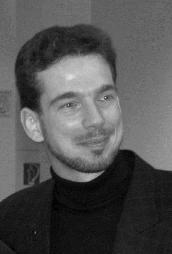
\includegraphics[width=0.7\linewidth]{bilder/magnor.jpg}\\
% 	Prof. Marcus Magnor
% \end{figure}

\nquestion{Welche Themenschwerpunkte m"ochten sie an Ihrem Institut bearbeiten?}

Visual Computing: Das steht f"ur alles, was sich um visuelle Informationsentstehung, -aufnahme, -verarbeitung, -analyse, -darstellung, und -wahrnehmung dreht. Das Spektrum unserer Forschungsthemen reicht von der Entwicklung von Bildanalyseverfahren z.B. f"ur Verkehrsszenen bis hin zu der Frage, warum ein Monet-Gem"alde eigentlich "asthetisch auf uns wirkt.

\nquestion{Was f"ur Pl"ane bezogen auf ihre T"atigkeit als Professor haben Sie?}

\begin{enumerate}
\item die Attraktivit"at des Informatikstudiums in Braunschweig weiter zu erh"ohen
\item das Forschungsprofil der Braunschweiger Informatik zu verst"arken
\item die internationale Sichtbarkeit der Braunschweiger Informatik weiter zu vergr"o"sern
\end{enumerate}

\nquestion{Wo sehen Sie sich in zehn Jahren?}

Inmitten meiner Gruppe von Mitarbeitern, die mit mir an L"osungen zu spannenden, aktuellen Forschungsfragen arbeiten.

\nquestion{Welche Herausforderungen kommen Ihrer Meinung nach in Zukunft auf die Informatik zu?}

\begin{itemize}
\item Moore's ,,Law'' wird eines nicht allzu fernen Tages seine G"ultigkeit verlieren.

- Trotzdem ist es uns noch nicht gelungen, die biologische Datenverarbeitung via Neuronen und Synapsen so zu verstehen, dass wir sie auch nur rudiment"ar nachmachen, geschweige denn nutzen k"onnten.

\item Das ,,Beamen'' (Teleportation) von Leuten funktioniert auch immer noch nicht \dots
\end{itemize}

\nquestion{Was w"urden Sie abschlie"send den Studierenden an dieser Stelle gerne mitteilen?}

carpe diem: Nehmen Sie alle Gelegenheiten wahr, die sich Ihnen bieten! 
